\subsection{Impedance Matching}

\begin{define}
    \textbf{Impedance:} the total resistance of a given electric component or AC circuit originating from reactive and resistance of the given system. Has both \textit{phase} and \textit{resistance} for AC. For DC, impedance has zero phase angle.

    \textbf{Impedance matching:} the process where the input impedance and the output impedance of a given electrical load are designed to reduce signal reflection and maximize the power transferred to the electric load.
\end{define}

\subsubsection{Motivation}
Impedance matching has great use in high-frequency and high-speed devices. 

When designing applications of ultra-high frequencies, impedance matching becomes a difficult operation for designers. The challenge is also reflected while designing microwaves and radio frequency circuits. When you get a wrong impedance matching, expect distorted pulses and high signal reflections.

An increase in frequency decreases the window of errors. The electrical circuit works the best when we have a perfectly matched impedance. If the impedance matching is not done, expect the system to work abnormally because of the effects such as the signal reflections. The reflected waves cause data delays and distortion of the phase and minimize the ratio of signal to noise.

\begin{concept}
    Maximum power transfer occurs when the resistance of the voltage source is equal to the resistance of the load.
\end{concept}

We can show this by taking the derivative of the power function. At maximum power transfer, this derivative is equal to zero
\subsubsection{Examples}
\begin{enumerate}
    \item Suppose that we have a system that is modeled by the circuit below
    \begin{center}
        \begin{circuitikz}[american]
            \draw (0,0)
            to[V, v=$V$, invert] (0,2)
            to[R, l=$R_{in}$, i=$i_{load}$] (2,2)
            to[R, l=$R_{load}$] (2,0)
            -- (0,0);
            \draw (2,2) -* (4,2) to[open, v=$V_{\text{out}}$] (4,0) -- (2,0);
        \end{circuitikz}    
    \end{center}
    \begin{align*}
        P &= I_{load}^2 R_{load} = \frac{V^2 R_{load}}{(R_{in} + R_{load})^2} \\
        \frac{dP}{dR_{load}} &= \frac{V^2(R_{in} + R_{load})^2 - 2R_{load}(R_{in} + R_{load})V^2}{(R_{in} + R_{load})^4} = 0 \Rightarrow R_{load} = R_{in}
    \end{align*}

    \item Suppose now you have the following circuit
        \begin{center}
            \begin{circuitikz}
                \draw (0,0)
                to[C, l=$C$] ++(0,2)
                to[L, l=$L$] ++(3,0)
                to[R, l=$R$] ++(0,-2)
                to (0,0);
            \end{circuitikz}
        \end{center}
        The admittance of the circuit, $Y_{in}$ is the inverse of the impedance. Here are the general steps for finding some $R'$ and $R$ such that their impedances matched
        \begin{enumerate}
            \item Calculate the impedance $Z$ of the circuit.
            \item Set admittance $Y = \frac{1}{Z}$.
            \item Separate your admittance into its real and imaginary part to take the real part of $Y$.
            \item $R' = \Re\{Y\}$, so that $R'$ here is a function of $R$.
        \end{enumerate}

    \textcolor{red}{i dont feel like doing the calculations right now im too tired do later though : \href{https://eepower.com/technical-articles/understanding-impedance-matching}{link}}

    \item \textbf{Transformer impedance matching:} set the turn ratio accordingly. Low voltage $\rightarrow$ fewer turns. 
        \begin{define}
            \[\text{Turns ratio }= \sqrt{\frac{\text{Source resistance}}{\text{Load resistance}}}\]
        \end{define}
    
    \item \textbf{Transmission line:} Transmission of electrical energy from the source to the load is done using a transmission line. While transferring this energy, it is important to zero or minimize energy losses that occur. For this to be possible, we should match the source and load impedances to the transmission line being used.
    
    The characteristic impedance is defined as the voltage and current wave ratio at any given point along the transmission line. If the transmission line in discussion is long, then we expect to have a different characteristic impedance at different distances along this transmission line. If we fail to do the impedance matching, the signs reaching the load will be reflected in the source of the origin, giving rise to a standing wave. The amount of power reflected is measured using the coefficient of reflection, which is calculated using the equation below
        \begin{define}
            \[\Gamma  = \frac{Z_L - Z_0}{Z_L + Z_0}\]
            $Z_L$: line impedance, $Z_0$: characteristic impedance
        \end{define}

    \item Attenna and television
        \begin{center}
            \begin{circuitikz}
                \draw (0,0)
                to[sV, v=$V_{in}$] ++(0,2)
                to[R, l=$R_A$] ++(3,0)
                to[R, l=$R_L$] ++(0,-2)
                to (0,0);
            \end{circuitikz}
        \end{center}
        $R_A$ is the resistance of the antenna is 150$\Omega$ and its cable while the TV's resistance is 600$\Omega$. Use the turns ratio formula to find the number of turns. Then set a transformer in between like in the image below.
        \begin{figure}[H]
            \centering
            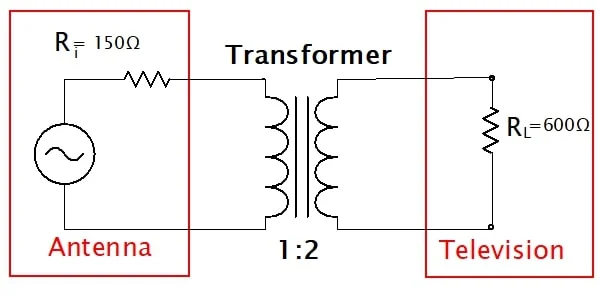
\includegraphics[scale=0.8]{figs/z_match_ex5.png}
        \end{figure}

    \item In the case of the headphone, the signal source is the device where the headphone is plugged. The headphone is the load. For the system to attain quality audio output, the source, and the load impedances must be matched. By matching the impedances, we make sure that there is maximum power transfer from the source of the audio to the headphone.

    When building portable devices, ensure that low-impedance headphones are built. This makes the system work well with proper sound quality.
\end{enumerate}


